\documentclass{beamer}

\usepackage{amsmath}
\usepackage{xspace}


% \newcommand\doubleplus{+\kern-1.3ex+\kern0.8ex}
\newcommand\doubleplus{\ensuremath{\mathbin{+\mkern-10mu+}}}


%% oracles
\newcommand{\ora}[1]{\ensuremath{\mathcal{O}\mathsf{#1}}\xspace}
%% algorithm
\newcommand{\algo}[1]{{\textsc{#1}}}
%%primitive algo
\newcommand{\primalgo}[1]{{\ensuremath{\mathsf{#1}}}\xspace}
%%primitive
\newcommand{\prim}[1]{{\ensuremath{\mathsf{#1}}}\xspace}
%%set
\newcommand{\setsym}[1]{{\ensuremath{\mathcal{#1}}}}
%%array
\newcommand{\arraysym}[1]{{\ensuremath{\mathsf{#1}}}}

\newcommand\N{\mathbb{N}}
\newcommand\F{\mathbb{F}}
% \newcommand\Gr{\mathbb{G}}


\def\mathperiod{.}
\def\mathcomma{.}



\newcommand*\set[1]{\{ #1 \}} % in text, we don't want {} to grow
\newcommand*\Set[1]{\left\{ #1 \right\}}
\newcommand*\setst[2]{\{ #1 | #2 \}}
\newcommand*\Setst[2]%
        {\left\{\,#1\vphantom{#2} \;\right|\left. #2 \vphantom{#1}\,\right\}}
% ``set such that''; puts in a vertical bar of the right height

\newcommand{\KeyGen}{\primalgo{KeyGen}}

% Why was this \prim before?
\newcommand{\VRF}{\primalgo{VRF}} 
\newcommand{\rVRF}{\primalgo{rVRF}} 

\newcommand{\Sign}{\primalgo{Sign}}
\newcommand{\Verify}{\primalgo{Verify}}
\newcommand{\Eval}{\primalgo{Eval}}
\newcommand{\Prove}{\primalgo{Prove}}
\newcommand{\Simulate}{\primalgo{Simulate}}
\newcommand{\Extract}{\primalgo{Extract}}


\newcommand{\In}{\primalgo{In}} 
\newcommand{\Out}{\primalgo{Out}} 
\newcommand{\PreOut}{\ensuremath{\primalgo{Out}_0}\xspace} 

\newcommand{\vk}{\ensuremath{\mathsf{vk}}\xspace}
\newcommand{\sk}{\ensuremath{\mathsf{sk}}\xspace}
\newcommand{\pk}{\ensuremath{\mathsf{pk}}\xspace}
\newcommand{\apk}{\ensuremath{\mathsf{apk}}\xspace}
\newcommand{\pkring}{\ensuremath{\setsym{PK}}}
\newcommand{\msg}{\ensuremath{\mathsf{msg}}\xspace}
\newcommand{\aux}{\ensuremath{\mathsf{aux}}\xspace}
\newcommand{\ctx}{\ensuremath{\mathsf{ctx}}\xspace}
\newcommand{\ringset}{\ensuremath{\mathsf{ring}}\xspace}



\newcommand\SNARK{\primalgo{SNARK}}
\newcommand\NIZK{\primalgo{NIZK}}


\newcommand{\adv}{\ensuremath{\mathcal{A}}\xspace}

\endinput

\newcommand{\evalprove}{\primalgo{EvalProve}}
\newcommand{\link}{{\primalgo{Link}}}
\newcommand{\update}{{\primalgo{Update}}}
\newcommand{\hashG}{\primalgo{H}_{\GG}}
\newcommand{\secreteval}{\primalgo{Secret}\eval}
\newcommand{\secretprove}{\primalgo{Secret}\prove}
\newcommand{\secretverify}{\primalgo{Secret}\verify}

\newcommand{\randsel}[0]{\ensuremath{\xleftarrow{\text{\$}}}}
\newcommand{\rel}{\ensuremath{\mathcal{R}}}


\endinput




\newcommand{\skvrf}{\ensuremath{\sk^{\mathsf{vrf}}}}
\newcommand{\pkvrf}{\ensuremath{\pk^{\mathsf{vrf}}}}
\newcommand{\skrvrf}{\ensuremath{\sk^{\mathsf{rvrf}}}}
\newcommand{\pkrvrf}{\ensuremath{\pk^{\mathsf{rvrf}}}}
\newcommand{\sksign}{\ensuremath{\sk^{\mathsf{sign}}}}
\newcommand{\pksign}{\ensuremath{\pk^{\mathsf{sign}}}}
\newcommand{\skksign}{\ensuremath{\sk^{\mathsf{kesign}}}}
\newcommand{\pkksign}{\ensuremath{\pk^{\mathsf{kesign}}}}
\newcommand{\pkssale}{\ensuremath{\pk^{\mathsf{ssale}}}}
\newcommand{\D}{\ensuremath{\Delta}}
\newcommand{\skzkvrf}{\ensuremath{\sk^{\mathsf{zkvrf}}}}
\newcommand{\pkzkvrf}{\ensuremath{\pk^{\mathsf{zkvrf}}}}


\def\comring{\ensuremath{\mathsf{comring}}\xspace}
\def\compk{\ensuremath{\mathsf{compk}}\xspace}


\title{Ethical identity, ring VRFs, and \\ zero-knowledge continuations}

\author{Jeffrey Burdges \and Handan Kilinc-Alper \and Alistair Stewart \and Sergey Vasilyev}
\date{15 Sept 2022}


\begin{document}


\maketitle



\begin{frame}
	
Ring signatures prove the actual signer exists in \\
\hspace{10pt} some publicly specified list, known as the ring.

\bigskip\bigskip

Examples:  Some deniable key exchanges, Monero, ZCash, etc.

\bigskip\bigskip

Ring can be a fancy set commitment like ZCash, \\
\hspace{10pt} but membership proofs are always very expensive.
	
\end{frame}



\begin{frame}{EC VRF}

A verifiable random function (VRF) proves evaluation of a pseudo-random function (PRF) determined by a signing key.

\bigskip\bigskip

$\mathsf{ECVRF}.\Verify(\msg,\aux,\pk,(\Out,R,R_\msg,s))$
	
$$ \begin{aligned}
\In &:= H_{\mathcal{G}}(\msg) \\
c &:= H(\msg,\aux,\pk,\Out,R,R_\msg) \\
s \, \In &= c \, \Out + R_\msg \\
s \, G &= c \, \pk + R \\
& \mathtt{return}\, H(\Out,\msg) \\
\end{aligned} $$
	
\end{frame}



\begin{frame}

Ring VRF is a ring signature that's also a VRF.

\bigskip\bigskip 

A ring verifiable random function (ring VRF) is a ring signature that proves evaluation of a pseudo-random function (PRF) determined by the actual key pair.

\end{frame}



\begin{frame}{Pedersen VRF}

We set $\compk := \sk \, G + b \, K$ to be a Pedersen commitment to $\sk$.

\bigskip\bigskip

$\mathsf{PedersenVRF}.\Verify(\msg,\aux,\compk,(\Out,R,R_\msg,s,t))$
	
$$ \begin{aligned}
\In &:= H_{\mathcal{G}}(\msg) \\
c &:= H(\msg,\aux,\pk,\Out,R,R_\msg) \\
s \, \In &= c \, \Out + R_\msg \\
t \, K + s \, G &= c \, \compk + R \\
& \mathtt{return} \, H(\Out,\msg) \\
\end{aligned} $$
	
\end{frame}



\begin{frame}
	
Zero-knowledge continuations..
	
\bigskip
	
Q: What are the fastest/cheapest SNARK proofs?
	
\bigskip
	
A: Ones we reuse without reproving.
	
\end{frame}



\begin{frame}

$\mathsf{Groth16}.\Verify(X,(A,B,C))$

$$ e(A,B) = e([\alpha]_1, [\beta]_2) \cdot e(X, [\gamma]_2) \cdot e(C, [\delta]_2) $$

\pause\medskip

$$ \begin{aligned}
 X &= \sk \, G + b \, K + \cdots \\
   &= \compk + \cdots \\
\end{aligned} $$

\pause\bigskip

Add $K_\delta := {\gamma\over\delta} K$ to trusted setup

$$ \begin{aligned}
X' &:= X + b K \\
A' &:= {1 \over r_1} A \\
B' &:= r_1 B + r_1 r_2 [\delta]_2 \\
C' &:= C + r_2 A + b K_\delta \\
\end{aligned} $$

\end{frame}



\begin{frame}

$X = \sk \, G + b \, K + \comring \, L$

\medskip

$$ \mathsf{Groth16} \Setst{ \sk_0 + \sk_1 2^{128}, \comring }{
    \exists d,o \textrm{\ s.t.\ }
	\genfrac{}{}{0pt}{}{ \sk_0 J_0 + \sk_1 J_1 + d J_2 }{ \in_o \comring }
} $$

\hspace{5pt} Marginal cost of eight $\mathcal{G}_1$ mults plus two $\mathcal{G}_2$ mults

\end{frame}
% \pause\bigskip\bigskip 



\begin{frame}
	
Avoid the Groth16 side channel..

\bigskip

$X = \sk \, G + b \, K + J_\pk.x \, L_x + J_\pk.y \, L_y$

\medskip

$$ \mathsf{Groth16} \Setst{ \sk_0 + \sk_1 2^{128}, J_\pk }{ 
	\exists d \textrm{\ s.t.\ }
	J_\pk = \sk_0 J_0 + \sk_1 J_1 + d J_2
} $$

\hspace{5pt} Use with hidden KZG opening of $J_\pk$ like Caulk/Caulk+

\end{frame}



\begin{frame} % {Identity}
	
Q: How can identity be safe for online use?

\bigskip

A: By revealing nothing except users' uniqueness.

\bigskip\bigskip

\hspace{10pt} No W3C attribute based bullshit!

\end{frame}



\begin{frame}{Identity}

Ring consists of people, with one key per person.

\bigskip\bigskip

User agent: \\ \medskip

1st) validates TLS cert of ``site.com'', including CT logs. \\ \medskip

2nd) sends ring VRF signature with $\msg = \mathtt{``site.com``}$. \\ \medskip

\pause\bigskip\bigskip 

What happens if we use $\msg = \mathtt{``site.com``} \doubleplus \mathsf{month}$?

\end{frame}



\begin{frame}

``No civilization can possibly survive to an interstellar spacefaring \\ \smallskip
\hspace{1pt} phase unless it limits its numbers'' (and its consumption) \\ \medskip
\hspace{1pt} --- Carl Sagan

\bigskip\bigskip 

We're headed for $+4^{\circ}$C so carrying capacity below 1 billion people.

\pause\bigskip\bigskip 

Anonymous rationing uses $\msg = \mathtt{``moutarde``} \doubleplus \mathsf{week} \doubleplus \mathsf{counter}$ \\
\hspace{1pt} And treats outputs as short lived nullifiers.

\bigskip\bigskip 

Also yields free-to-play games, promotional discounts, etc.

\end{frame}



\begin{frame}

As fraudulent TLS and covid certificates are commonplace..

\bigskip

Q: How can ration cards be trusted?

\bigskip 

A: By asking users trust a public list of residents, not certificates.

% Important: Ring membership can be transparent!  No fraudulent certificates!

\end{frame}



\begin{frame}{Sassafras}

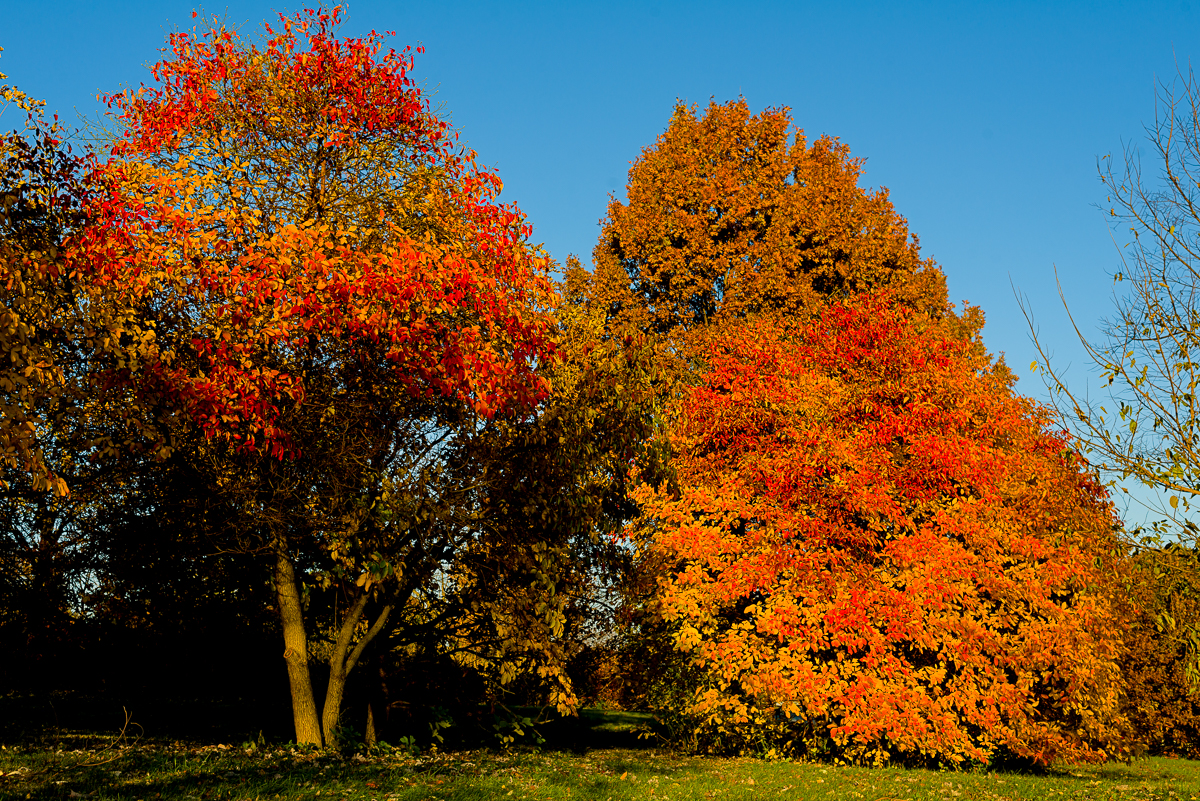
\includegraphics[width=\textwidth]{Sassafras-albidum.jpg}

\end{frame}



\begin{frame}

Sassafras: Semi-anonymous sortition of staked assignees \\
\hspace{5pt} for fixed-time rhythmic assignment of slots

\bigskip

It's a (semi) secret single leader election (semi-SSLE) \\
\hspace{5pt} by cards against humanity.

\bigskip

% black_FRONT050.png

\begin{columns}
	\begin{column}[t]{0.1\textwidth}
	\end{column}
	\begin{column}[t]{0.3\textwidth}
		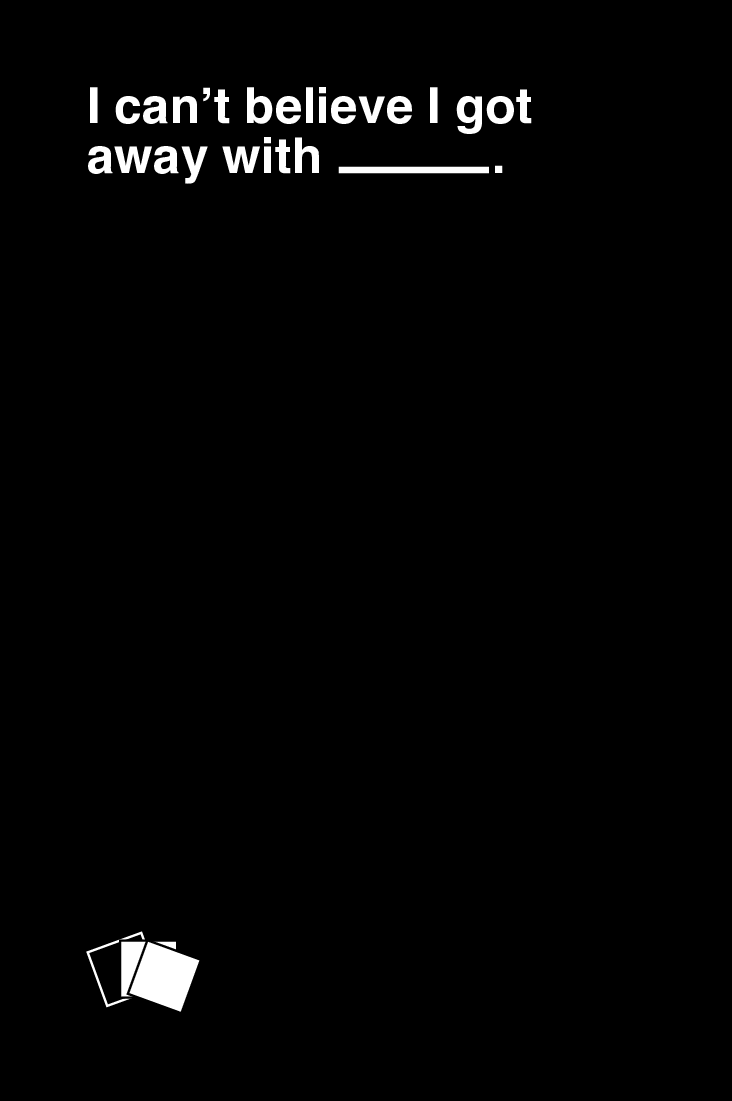
\includegraphics[width=.9\textwidth]{black_FRONT012.png} % {CAC/PNGs-to-print/individual-cards/black_FRONT012.png}
	\end{column}
	\begin{column}[t]{0.3\textwidth}
		\frame{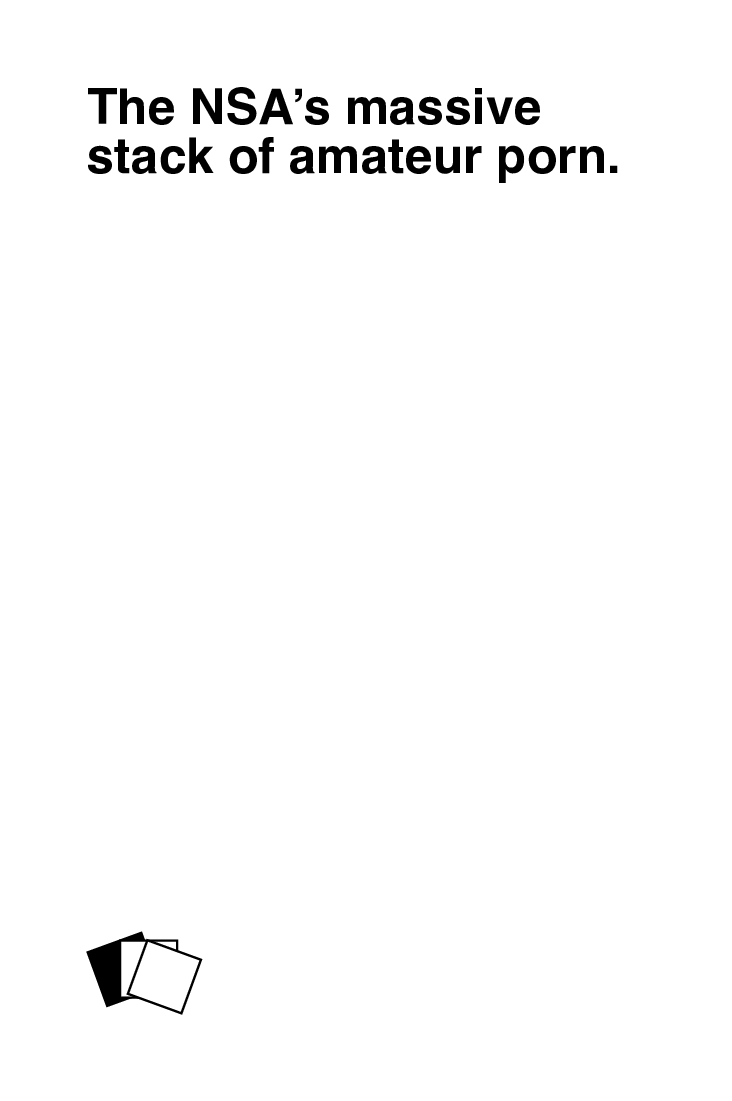
\includegraphics[width=.9\textwidth]{white_FRONT227.png}} % {CAC/PNGs-to-print/individual-cards/white_FRONT227.png}
	\end{column}
	\begin{column}[t]{0.3\textwidth}
	    \frame{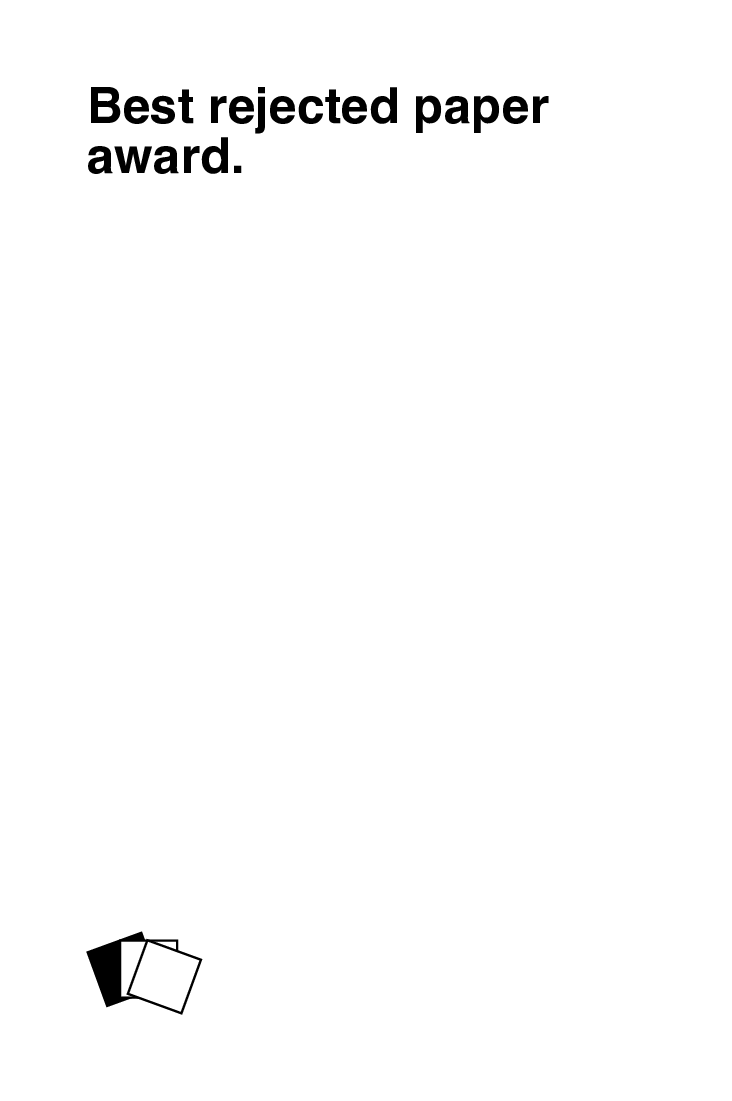
\includegraphics[width=.9\textwidth]{white_FRONT117.png}} % {CAC/PNGs-to-print/individual-cards/black_FRONT050.png}
    \end{column}
\end{columns}


\end{frame}



\begin{frame}{Sassafras}

Disadvantages: \\
- Network layer anonymity is weak, but we not care much.. \\

\bigskip\bigskip

Advantages: \\ \smallskip
- Ouroboros Praos quality randomness \\ \smallskip
- Vastly more efficient than Boneh's shuffle SSLEs \\ \smallskip
- Block producers can prove their slot in advance \\ \smallskip
- Users send tx to upcoming slots via Tor-like {.onion} circuits. \\ \smallskip
% Tor-like {.onion} circuit to upcoming slots \\
%  \hspace{5pt} so users can sent tx directly to upcoming slots. \\ \smallskip
- Avoids need for memepools, saving bandwidth and CPU. \\ \smallskip
- Better MEV defenses \\ \smallskip

\pause\bigskip\bigskip

\hspace{10pt} Smart contracts, the Ford Pinto of security.

\end{frame}



\end{document}





\begin{frame}
		
\end{frame}



\begin{frame}
	
\end{frame}




